% %%%%%%%%%%%%%%%%%%%%%%%%%%%%%%%%%%%%%%%%%%%%%%%%%%%%%%%%%%%%%%%%%%%%%%%%%%%%%
% %%%%%%%%%%%%%%%%%%%%%%%%%%%%%%%%%%%%%%%% Survey of the Near-Earth Environment
% %%%%%%%%%%%%%%%%%%%%%%%%%%%%%%%%%%%%%%%%%%%%%%%%%%%%%%%%%%%%%%%%%%%%%%%%%%%%%

\chapter{From the Sun to the Earth}
\label{ch_intro}

It's all about energy transfer! 

Some example citations, including a few with special characters: \cite{dai_2013}, \cite{dai_2015}, \cite{lysak_2001}. 

%There are a lot of interrelated things going on, so it's hard to describe Earth's environment one step at a time. Look at Scott's thesis -- he did this well, right? 

%Heliosphere, Magnetosphere, Ionosphere, Atmosphere?

%Current systems, convective systems, density profiles? 

\begin{figure}
  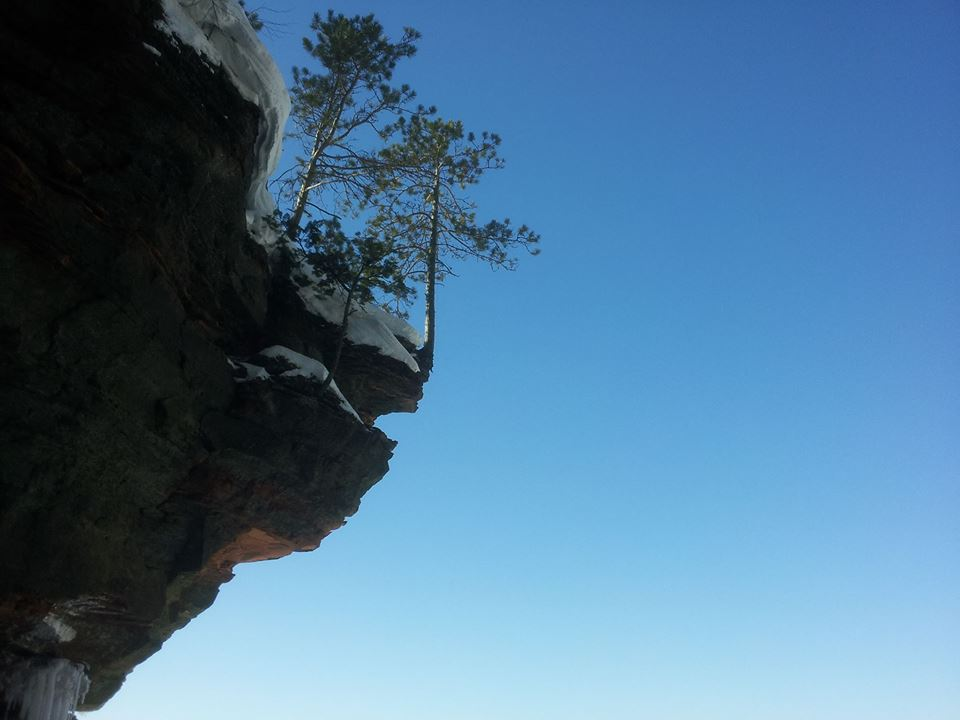
\includegraphics[width=5.75in, height=2in]{figures/image.jpg}
  \caption{Lorem ipsum dolor sit amet, consectetur adipiscing elit, sed do eiusmod tempor incididunt ut labore et dolore magna aliqua.}
  \label{fig_test}
\end{figure}

Talking about the solar wind... maybe even a big about the solar dynamo. 


% =============================================================================
% =============================================================================
% =============================================================================
\section{The Outer Magnetosphere}

\subsection{The Magnetopause}

\subsection{The Magnetotail}

\subsection{Cusp Regions}

% =============================================================================
% =============================================================================
% =============================================================================
\section{The Inner Magnetosphere}

Characteristic profiles for $\omega_P$, $\Omega$, $v_A$, $\sigma$, $\epsilon$...

Table: bounce times as a function of L. How much does this depend on day vs night, storm vs calm? 

\subsection{The Plasmasphere}

\subsection{Ring Currents}

\subsection{The Radiation Belts}

% =============================================================================
% =============================================================================
% =============================================================================
\section{Geomagnetic Disturbances}

\subsection{Storms}

\subsection{Substorms}






